\documentclass{article}\usepackage[]{graphicx}\usepackage[]{color}
%% maxwidth is the original width if it is less than linewidth
%% otherwise use linewidth (to make sure the graphics do not exceed the margin)
\makeatletter
\def\maxwidth{ %
  \ifdim\Gin@nat@width>\linewidth
    \linewidth
  \else
    \Gin@nat@width
  \fi
}
\makeatother

\definecolor{fgcolor}{rgb}{0.345, 0.345, 0.345}
\newcommand{\hlnum}[1]{\textcolor[rgb]{0.686,0.059,0.569}{#1}}%
\newcommand{\hlstr}[1]{\textcolor[rgb]{0.192,0.494,0.8}{#1}}%
\newcommand{\hlcom}[1]{\textcolor[rgb]{0.678,0.584,0.686}{\textit{#1}}}%
\newcommand{\hlopt}[1]{\textcolor[rgb]{0,0,0}{#1}}%
\newcommand{\hlstd}[1]{\textcolor[rgb]{0.345,0.345,0.345}{#1}}%
\newcommand{\hlkwa}[1]{\textcolor[rgb]{0.161,0.373,0.58}{\textbf{#1}}}%
\newcommand{\hlkwb}[1]{\textcolor[rgb]{0.69,0.353,0.396}{#1}}%
\newcommand{\hlkwc}[1]{\textcolor[rgb]{0.333,0.667,0.333}{#1}}%
\newcommand{\hlkwd}[1]{\textcolor[rgb]{0.737,0.353,0.396}{\textbf{#1}}}%
\let\hlipl\hlkwb

\usepackage{framed}
\makeatletter
\newenvironment{kframe}{%
 \def\at@end@of@kframe{}%
 \ifinner\ifhmode%
  \def\at@end@of@kframe{\end{minipage}}%
  \begin{minipage}{\columnwidth}%
 \fi\fi%
 \def\FrameCommand##1{\hskip\@totalleftmargin \hskip-\fboxsep
 \colorbox{shadecolor}{##1}\hskip-\fboxsep
     % There is no \\@totalrightmargin, so:
     \hskip-\linewidth \hskip-\@totalleftmargin \hskip\columnwidth}%
 \MakeFramed {\advance\hsize-\width
   \@totalleftmargin\z@ \linewidth\hsize
   \@setminipage}}%
 {\par\unskip\endMakeFramed%
 \at@end@of@kframe}
\makeatother

\definecolor{shadecolor}{rgb}{.97, .97, .97}
\definecolor{messagecolor}{rgb}{0, 0, 0}
\definecolor{warningcolor}{rgb}{1, 0, 1}
\definecolor{errorcolor}{rgb}{1, 0, 0}
\newenvironment{knitrout}{}{} % an empty environment to be redefined in TeX

\usepackage{alltt}

\usepackage{fancyhdr} % Required for custom headers
\usepackage{lastpage} % Required to determine the last page for the footer
\usepackage{extramarks} % Required for headers and footers
\usepackage{graphicx} % Required to insert images
\usepackage{hyperref}
\usepackage{amsmath} %for binomial pdf
\usepackage{parskip} % so that there's space bw paragraphs
\usepackage{float}
\usepackage{amsfonts}

% Margins
\topmargin=-0.45in
\evensidemargin=0in
\oddsidemargin=0in
\textwidth=6.5in
\textheight=9.0in
\headsep=0.25in 

\linespread{1.1} % Line spacing

% Set up the header and footer
\pagestyle{fancy}
\lhead{STAT 534: Spatial} % Top left header
\chead{HW 2} % Top center header
\rhead{Andrea Mack} % Top right header
\lfoot{01/30/2017} % Bottom left footer
\cfoot{} % Bottom center footer
\rfoot{Page\ \thepage\ of\ \pageref{LastPage}} % Bottom right footer
\renewcommand\headrulewidth{0.4pt} % Size of the header rule
\renewcommand\footrulewidth{0.4pt} % Size of the footer rule

\setlength\parindent{0pt} % Removes all indentation from paragraphs
\setlength\parskip{0.5cm}
\restylefloat{table}

%----------------------------------------------------------------------------------------
%	DOCUMENT STRUCTURE COMMANDS
%	Skip this unless you know what you're doing
%----------------------------------------------------------------------------------------

% Header and footer for when a page split occurs within a problem environment
\newcommand{\enterProblemHeader}[1]{
\nobreak\extramarks{#1}{#1 continued on next page\ldots}\nobreak
\nobreak\extramarks{#1 (continued)}{#1 continued on next page\ldots}\nobreak
}

% Header and footer for when a page split occurs between problem environments
\newcommand{\exitProblemHeader}[1]{
\nobreak\extramarks{#1 (continued)}{#1 continued on next page\ldots}\nobreak
\nobreak\extramarks{#1}{}\nobreak
}


%----------------------------------------------------------------------------------------%
\IfFileExists{upquote.sty}{\usepackage{upquote}}{}
\begin{document}



\begin{enumerate}
\item {\it It was pointed out in class that, conditional on n events, event locations are uniformly dis- tributed for a homogeneous Poisson process. We will consider the simplest example of this. Consider a one-dimensional process on a transect of length L, (0,L]. Given that one event has occurred on the interval (0, L] what is the probability that it occurred in the subinterval (0, s] for s \textless L?}

\vspace{2in}

\item {\it We looked at an example of quadrat.test on the amacrine data set in class. We will use it to analyze another data set, called redwood. You can read about this in the spatstat help material. You will be using the quadrat.test function. You can also read about this function in the help material.}

\begin{enumerate}
\item {\it Read the help pages on the quadrat.test function. What null hypothesis do they claim to be testing?}

The help page for {\texttt quadrat.test} suggest $H_{0}$ is complete spatial randomness for a given point pattern.

\item {\it Use quadrat.test on the redwood data set.}

\begin{knitrout}\footnotesize
\definecolor{shadecolor}{rgb}{0.969, 0.969, 0.969}\color{fgcolor}\begin{kframe}


{\ttfamily\noindent\color{warningcolor}{Warning: Some expected counts are small; chi\textasciicircum{}2 approximation may be inaccurate}}\end{kframe}

{\centering 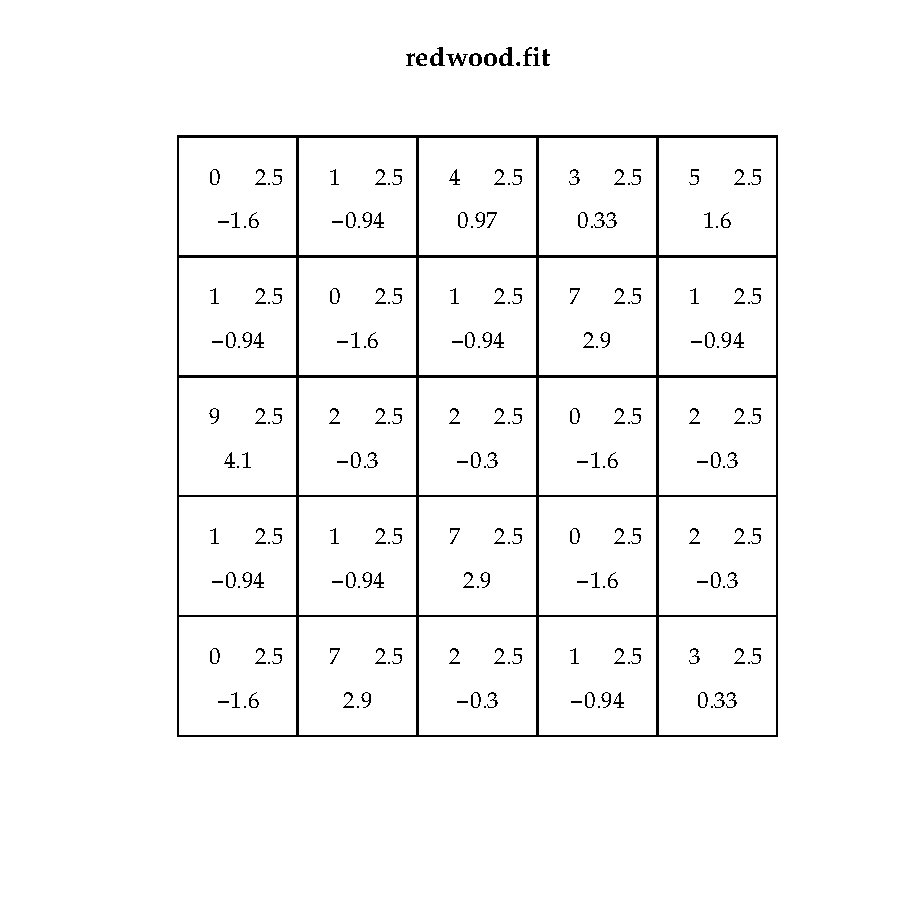
\includegraphics[width=\maxwidth]{figure/prob2b-1} 

}


\begin{kframe}\begin{verbatim}

	Chi-squared test of CSR using quadrat counts
	Pearson X2 statistic

data:  redwood
X2 = 64.613, df = 24, p-value = 2.774e-05
alternative hypothesis: two.sided

Quadrats: 5 by 5 grid of tiles
\end{verbatim}
\end{kframe}
\end{knitrout}

{\it The default partitioning of the grid is 5 × 5. Does that appear appropriate here? Justify your answer.}

It was recommended to have at least 5 observations in each grid cell when using the $\chi^{2}$ distribution to approximate the p-value. Several cells have less than two seedleeings or saplings and so the 5X5 grid is not appropriate. A warning message also indicates the low cell count is a problem.

\item {\it Redo the analysis using a 3 × 3 grid.}

Using the 3X3 grid cell counts seem to be adequate to use the the $\chi^{2}$ distribution.

\begin{knitrout}\footnotesize
\definecolor{shadecolor}{rgb}{0.969, 0.969, 0.969}\color{fgcolor}\begin{kframe}
\begin{verbatim}

	Chi-squared test of CSR using quadrat counts
	Pearson X2 statistic

data:  redwood
X2 = 22.774, df = 8, p-value = 0.007333
alternative hypothesis: two.sided

Quadrats: 3 by 3 grid of tiles
\end{verbatim}
\end{kframe}
\end{knitrout}

\item {\it Is the value of the test statistic $X^2$ indicative of clustering, CSR, or a regular pattern? Justify your answer. Note that I am only asking you to compare the observed value of $X^2$ to what you would expect under each of these three patterns. You do not need to calculate a P-value just yet.}

The value of the $\chi^{2}_{8}$ test statistic is 22.8 which suggests spatial clustering. A test statistic of 8 is indicative of CSR (though that cannot be proved) and a test statistic below 8 is indicative of regularity.

{\it The investigator suspected a clustered pattern and the plot would seem to be consistent with this. Rerun the test with alternative=``c" in the argument list. Give the p-value for the test and interpret the results. Does the test provide evidence against CSR and for clustering? Justify your answer.}


The default alternative hypothesis is a two sided. Based on a p-value of 0.00367, there is strong evidence against CSR and for spatial clustering. 


\item {\it We can plot the results of the fit.}

{\it You will see a plot of the 3 × 3 grid. There are 3 numbers in each cell: the observed count (upper left), expected count under CSR (upper right), and a scaled residual (lower number). The sum of the scaled residuals is the $\chi^{2}$ statistic. Give the results of the test and using the plot indicate where CSR seems to break down, if it does.}

\begin{knitrout}\footnotesize
\definecolor{shadecolor}{rgb}{0.969, 0.969, 0.969}\color{fgcolor}

{\centering 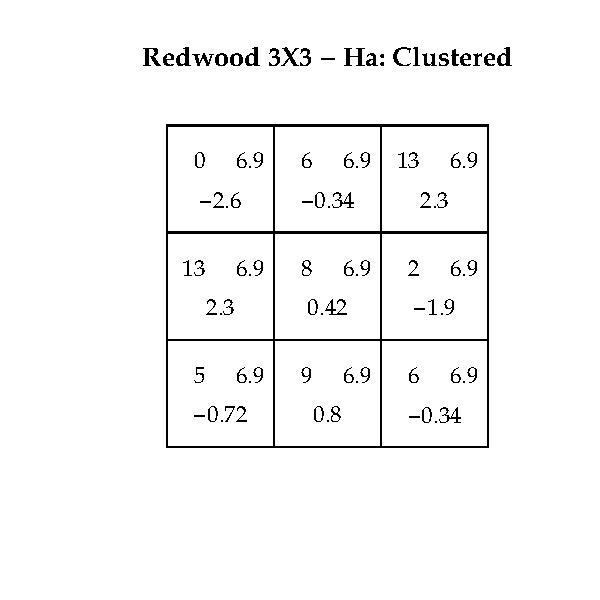
\includegraphics[width=\maxwidth]{figure/prob3f-1} 

}



\end{knitrout}

The observed $\chi^{2}$ statistic was 22.774 which resulted in a p-value of 0.00367 when compared to a $\chi^{2}_{8}$ distribution. There is strong evidence of spatial clustering. CSR appears to break down in cells (1,1); (2,1); (1,3); (2,3) as there is a large discrepancy between the expected and oberved cell counts. The scaled residuals are also larger in these cells. Note that under CSR, the expected cell counts are all the same. and spatial clustering is suggested (vs. regularity) because the cells have large discrepancies. Under regularity, there would be very little if no difference betwen the observed and expected counts. 

\item {\it Quadrat size can be important. Repeat the analysis using a 2X2 grid. Give the results and compare to what we saw with the 3 × 3 grid.}



Using a 2X2 grid, a $\chi^{2}_{3}$ test statistic of 6.52 resulted in a p-value of 0.089. There is some evidence against CSR and for spaital clustering of the seedlings.

There is less evidence for spatial clustering when using the 2X2 grid than using the 3X3 grid. As the number of cells decrease, it is less likely to see more discrepancies.


\end{enumerate}

\item {\it We will compare results from Monte Carlo procedures based on Poisson sampling and based on conditioning on the number of observed points. We will use the cells data set. The R code to accomplish that is shown below. Compare the two procedures. What do they indicate about the spatial pattern and why? Which procedure do you like best for this data set and why?}

Both procedures indicate the observed average nearest neighbor distance is much farther than would be expected under CSR and is indicative of spatial regularity.

\begin{knitrout}\footnotesize
\definecolor{shadecolor}{rgb}{0.969, 0.969, 0.969}\color{fgcolor}

{\centering 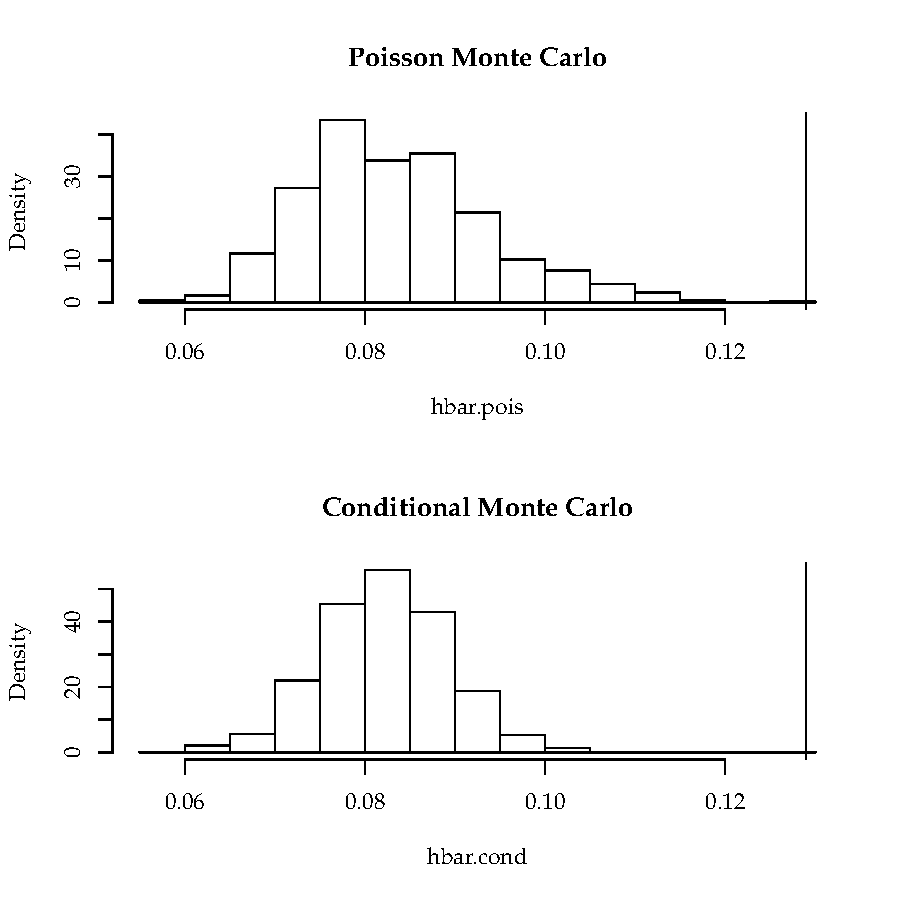
\includegraphics[width=\maxwidth]{figure/prob3-1} 

}



\end{knitrout}
  
\begin{knitrout}\footnotesize
\definecolor{shadecolor}{rgb}{0.969, 0.969, 0.969}\color{fgcolor}

{\centering 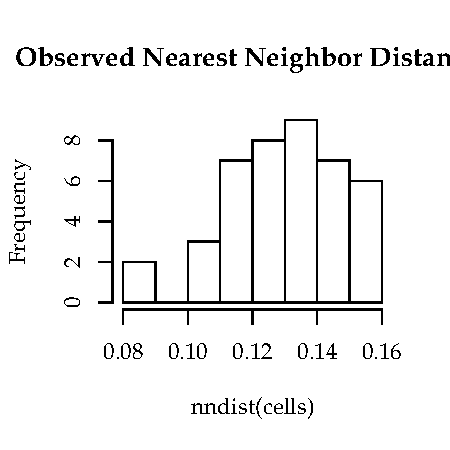
\includegraphics[width=\maxwidth]{figure/another-1} 

}



\end{knitrout}
  
I prefer the Conditional Monte Carlo procedure here because the simulated distribution is symmetric. 


\item {\it Below is the frequency distribution of the number of trees per quadrat in a sample of 100 quadrats each of radius 6 m.
}

{\it The data were pooled for counts ≥ 5 to meet the assumptions of the method. Carry out a Poisson goodness-of-fit test based on an assumption of CSR. Discuss the results. The sample mean of the observed counts was 1.43.
}

A Poisson goodness of fit test was carried to assess evidence against a CSR process modeled by a Poisson(1.43) distribution. The formal hypothese are below:

$H_{o}$: The distribution of counts is Poisson(1.43)

$H_{a}$: The distribution of counts is not Poisson(1.43)

% latex table generated in R 3.3.2 by xtable 1.8-2 package
% Fri Jan 27 11:47:32 2017
\begin{table}[ht]
\centering
\begin{tabular}{||l|l|l|l|l|l|l||}
  \hline
 & 0 & 1 & 2 & 3 & 4 & at least 5 \\ 
  \hline
Expected & 23.93 & 34.22 & 24.47 & 11.66 & 4.17 & 1.55 \\ 
  Observed & 34.00 & 33.00 & 17.00 & 7.00 & 3.00 & 6.00 \\ 
   \hline
\end{tabular}
\end{table}

  
  The observed data resulted in a $\chi^{2}$ test statistic of 21.569. Comparing the test statistic to a $\chi^{2}_{4}$ distribution resulted in a p-value of \ensuremath{6\times 10^{-4}}. There is some evidence against the distribution of seedlings being Poisson(1.43).
  
  Clustering vs. regularity must be established by looking at the data. The expected counts are more distant than the observed counts which suggests clustering.
  
   \item {\it Suppose we have a realization of a spatial point process consisting of N event locations {s1, s2, · · · , sN }. Let Hi denote the distance between the ith event and the nearest neighboring event. The cumulative distribution function of H (the nearest event-event distance) is the G function. (This problem will be continued on the next homework assignment).}
  
  \begin{enumerate}
  \item {\it What is the G function if the point process is CSR; i.e. what is G(h) = P (H $\leq$ h) ?}
  
  \vspace{1in}
  
  \item {\it Find the pdf of H.}
  
  \vspace{2in}
  
  \item {\it Find E[H] and Var(H). Hint: you found the pdf but before you start evaluating a gnarly integral take a close look at that pdf and see if you cannot identify the family of distributions it belongs to. If you can do that then you can use that knowledge to find the mean and variance.}
  
\end{enumerate}
\end{enumerate}
\end{document}

